%% BioMed_Central_Tex_Template_v1.06
%%                                      %
%  bmc_article.tex            ver: 1.06 %
%                                       %

%%IMPORTANT: do not delete the first line of this template
%%It must be present to enable the BMC Submission system to 
%%recognise this template!!

%%%%%%%%%%%%%%%%%%%%%%%%%%%%%%%%%%%%%%%%%
%%                                     %%
%%  LaTeX template for BioMed Central  %%
%%     journal article submissions     %%
%%                                     %%
%%         <14 August 2007>            %%
%%                                     %%
%%                                     %%
%% Uses:                               %%
%% cite.sty, url.sty, bmc_article.cls  %%
%% ifthen.sty. multicol.sty		   %%
%%				      	   %%
%%                                     %%
%%%%%%%%%%%%%%%%%%%%%%%%%%%%%%%%%%%%%%%%%


%%%%%%%%%%%%%%%%%%%%%%%%%%%%%%%%%%%%%%%%%%%%%%%%%%%%%%%%%%%%%%%%%%%%%
%%                                                                 %%	
%% For instructions on how to fill out this Tex template           %%
%% document please refer to Readme.pdf and the instructions for    %%
%% authors page on the biomed central website                      %%
%% http://www.biomedcentral.com/info/authors/                      %%
%%                                                                 %%
%% Please do not use \input{...} to include other tex files.       %%
%% Submit your LaTeX manuscript as one .tex document.              %%
%%                                                                 %%
%% All additional figures and files should be attached             %%
%% separately and not embedded in the \TeX\ document itself.       %%
%%                                                                 %%
%% BioMed Central currently use the MikTex distribution of         %%
%% TeX for Windows) of TeX and LaTeX.  This is available from      %%
%% http://www.miktex.org                                           %%
%%                                                                 %%
%%%%%%%%%%%%%%%%%%%%%%%%%%%%%%%%%%%%%%%%%%%%%%%%%%%%%%%%%%%%%%%%%%%%%


\documentclass[10pt]{article}    



% Load packages
\usepackage{cite} % Make references as [1-4], not [1,2,3,4]
\usepackage{url}  % Formatting web addresses  
\usepackage{ifthen}  % Conditional 
\usepackage{multicol}   %Columns
\usepackage{hhline}
\usepackage[utf8]{inputenc} %unicode support
\usepackage{graphicx}
\usepackage{verbatim}
%\usepackage[applemac]{inputenc} %applemac support if unicode package fails
%\usepackage[latin1]{inputenc} %UNIX support if unicode package fails
\urlstyle{rm}
 
 
%%%%%%%%%%%%%%%%%%%%%%%%%%%%%%%%%%%%%%%%%%%%%%%%%	
%%                                             %%
%%  If you wish to display your graphics for   %%
%%  your own use using includegraphic or       %%
%%  includegraphics, then comment out the      %%
%%  following two lines of code.               %%   
%%  NB: These line *must* be included when     %%
%%  submitting to BMC.                         %% 
%%  All figure files must be submitted as      %%
%%  separate graphics through the BMC          %%
%%  submission process, not included in the    %% 
%%  submitted article.                         %% 
%%                                             %%
%%%%%%%%%%%%%%%%%%%%%%%%%%%%%%%%%%%%%%%%%%%%%%%%%                     


%\def\includegraphic{}
%\def\includegraphics{}



\setlength{\topmargin}{0.0cm}
\setlength{\textheight}{21.5cm}
\setlength{\oddsidemargin}{0cm} 
\setlength{\textwidth}{16.5cm}
\setlength{\columnsep}{0.6cm}


%%%%%%%%%%%%%%%%%%%%%%%%%%%%%%%%%%%%%%%%%%%%%%%%%%
%%                                              %%
%% You may change the following style settings  %%
%% Should you wish to format your article       %%
%% in a publication style for printing out and  %%
%% sharing with colleagues, but ensure that     %%
%% before submitting to BMC that the style is   %%
%% returned to the Review style setting.        %%
%%                                              %%
%%%%%%%%%%%%%%%%%%%%%%%%%%%%%%%%%%%%%%%%%%%%%%%%%%
 

%Review style settings
%\newenvironment{bmcformat}{\begin{raggedright}\baselineskip20pt\sloppy\setboolean{publ}{false}}{\end{raggedright}\baselineskip20pt\sloppy}

%Publication style settings
%\newenvironment{bmcformat}{\fussy\setboolean{publ}{true}}{\fussy}

%New style setting

% Begin ...
\begin{document}


%%%%%%%%%%%%%%%%%%%%%%%%%%%%%%%%%%%%%%%%%%%%%%
%%                                          %%
%% Enter the title of your article here     %%
%%                                          %%
%%%%%%%%%%%%%%%%%%%%%%%%%%%%%%%%%%%%%%%%%%%%%%

%\title{A Probablistic Space-efficient Method of Obtaining Solid Kmers with An Appliction of Error Correction}
\title{Lighter: fast and memory-efficient error correction without counting}

%%%%%%%%%%%%%%%%%%%%%%%%%%%%%%%%%%%%%%%%%%%%%%
%%                                          %%
%% Enter the authors here                   %%
%%                                          %%
%% Ensure \and is entered between all but   %%
%% the last two authors. This will be       %%
%% replaced by a comma in the final article %%
%%                                          %%
%% Ensure there are no trailing spaces at   %% 
%% the ends of the lines                    %%     	
%%                                          %%
%%%%%%%%%%%%%%%%%%%%%%%%%%%%%%%%%%%%%%%%%%%%%%


\author{Li Song$^1$%
       Liliana Florea$^2$
      Ben Langmead$^{*3}$ %
      }
\date{}     

%%%%%%%%%%%%%%%%%%%%%%%%%%%%%%%%%%%%%%%%%%%%%%
%%                                          %%
%% Enter the authors' addresses here        %%
%%                                          %%
%%%%%%%%%%%%%%%%%%%%%%%%%%%%%%%%%%%%%%%%%%%%%%

\maketitle

%%%%%%%%%%%%%%%%%%%%%%%%%%%%%%%%%%%%%%%%%%%%%%
%%                                          %%
%% The Abstract begins here                 %%
%%                                          %%  
%% Please refer to the Instructions for     %%
%% authors on http://www.biomedcentral.com  %%
%% and include the section headings         %%
%% accordingly for your article type.       %%   
%%                                          %%
%%%%%%%%%%%%%%%%%%%%%%%%%%%%%%%%%%%%%%%%%%%%%%


\begin{abstract}
        % Do not use inserted blank lines (ie \\) until main body of text.
\emph{Lighter} is a fast and memory-efficient tool for correcting sequencing errors in high-throughput sequencing datasets.
\emph{Lighter} avoids counting $k$-mers in the sequencing reads.
Instead, it uses a pair of Bloom filters, one populated with a sample of the input $k$-mers and the other populated with $k$-mers likely to be correct based on a statistical test.
As long as the sampling fraction is adjusted proportionally to the dataset's average coverage, the Bloom filter size can be held constant while maintaining near-constant occupancy and false positive rate.
\emph{Lighter} is easily applied to very large sequencing datasets.  It uses no secondary storage, and is both faster and more memory-efficient than competing approaches while achieving comparable accuracy.
\emph{Lighter} is free open source software available from \url{https://github.com/mourisl/Lighter/}.
\end{abstract}


%%%%%%%%%%%%%%%%%%%%%%%%%%%%%%%%%%%%%%%%%%%%%%
%%                                          %%
%% The Main Body begins here                %%
%%                                          %%
%% Please refer to the instructions for     %%
%% authors on:                              %%
%% http://www.biomedcentral.com/info/authors%%
%% and include the section headings         %%
%% accordingly for your article type.       %% 
%%                                          %%
%% See the Results and Discussion section   %%
%% for details on how to create sub-sections%%
%%                                          %%
%% use \cite{...} to cite references        %%
%%  \cite{koon} and                         %%
%%  \cite{oreg,khar,zvai,xjon,schn,pond}    %%
%%  \nocite{smith,marg,hunn,advi,koha,mouse}%%
%%                                          %%
%%%%%%%%%%%%%%%%%%%%%%%%%%%%%%%%%%%%%%%%%%%%%%

% The idea of using a Bloom filter to store the solid k-mers is not new; CUDA-EC does this
% What's our story w/r/t choosing k-mer length?

\section*{Introduction}
The cost and throughput of DNA sequencing have improved very rapidly in the past several years \cite{glenn2011field}.
Recent advances have reduced the cost of sequencing a single human genome at 30-fold coverage to around \$1,000 \cite{1kgenomeforreal}.
Consequently, there has been an explosion of new software for analyzing large collections of sequencing reads.
Correction of sequencing errors is a basic need in many of these tools.
Removing errors at the outset can improve speed, memory-efficiency and accuracy of downstream tools \cite{kelley2010quake}.
This is particularly true for analyses involving de novo assembly with De Bruijn graphs, since the size of the graph increases with the number of distinct $k$-mers in the dataset \cite{pevzner2001eulerian, chaisson2004fragment}.

For an error correction tools to be truly usable, time and memory requirements must be very modest.
When input datasets are extremely large (e.g. billions of reads), and when the genome under study is large (e.g. human), this challenge is particularly pronounced.

%One important way to study a species is to sequence its genome and analyze its DNA. The need to understand the genome stimulates the rapid development of DNA sequencing technologies. The output of the DNA sequencing is usually an enormous volume of short fragments from the genome. With these small fragments, computational biologists are able to design complicated methods to reconstruct the original genome by assembling or to detect the mutations from the known reference genome by aligning.

The volume of the data is so huge that if we align them to the genome, each position is covered by a bunch of reads which is called the coverage. However, the short fragments are not perfect and usually contain a small number of sequecing errors. This affects one of the most important preprocessing stages for the data --- kmer counting, where a kmer is a nucleutide sequence of size k. If there is no sequencing error, all the kmers are from the genome, which are called solid kmers, and its quantity are bounded by the genome size instead of the coverage. This is not true in practice due to the sequecing errors and if the coverage is high enough, like what the sequecing technology gives us nowadays, the kmers containing sequencing errors will dominate the space consumption. To alleviate the impact from those non-solid kmers, various methods have been proposed, like BFcounter[cite]. These methods still suffer from the problem that the space consumption scales up with the coverage. In this paper, we propose a probablitic methods of obtaining solid kmers whose space complexity does not depend on the coverage.

One immediate applicaiton using the information of solid kmers is error correction. Error correction is very important for the De Brujin graph based genome assemblers to save the memory usage. There are mainly three categories methods for error correction[cite], and converting all the kmers to solid kmers is one of them and is particularly successful for Illumina reads where the read errors are mainly substitutions. There are currently many programs for error corrections, and some of them are highlighted for their low memory usage, like Musket[cite] and Bless[cite]. With the help of our method of obtainig solid kmers and the bloom filters which is a compact probabilitc data structure, we also propose the program Lighter(LIGHT-weight ERror correction) that can do error correction with very small memory footprint and no extra disk consumption.

\section*{Method}
Lighter's workflow is illustrated in Figure \ref{fig:lighter_framework}. Lighter makes three passes over the input reads.  The first pass obtains a sample of the k-mers present in the input reads, storing the sample in Bloom filter A.  The second pass uses Bloom filter A to identify ``solid'' k-mers and stores these in Bloom filter B.  The third pass uses Bloom filter B to detect and correct errors in the input reads.

\begin{figure}[h!]
\begin{center}
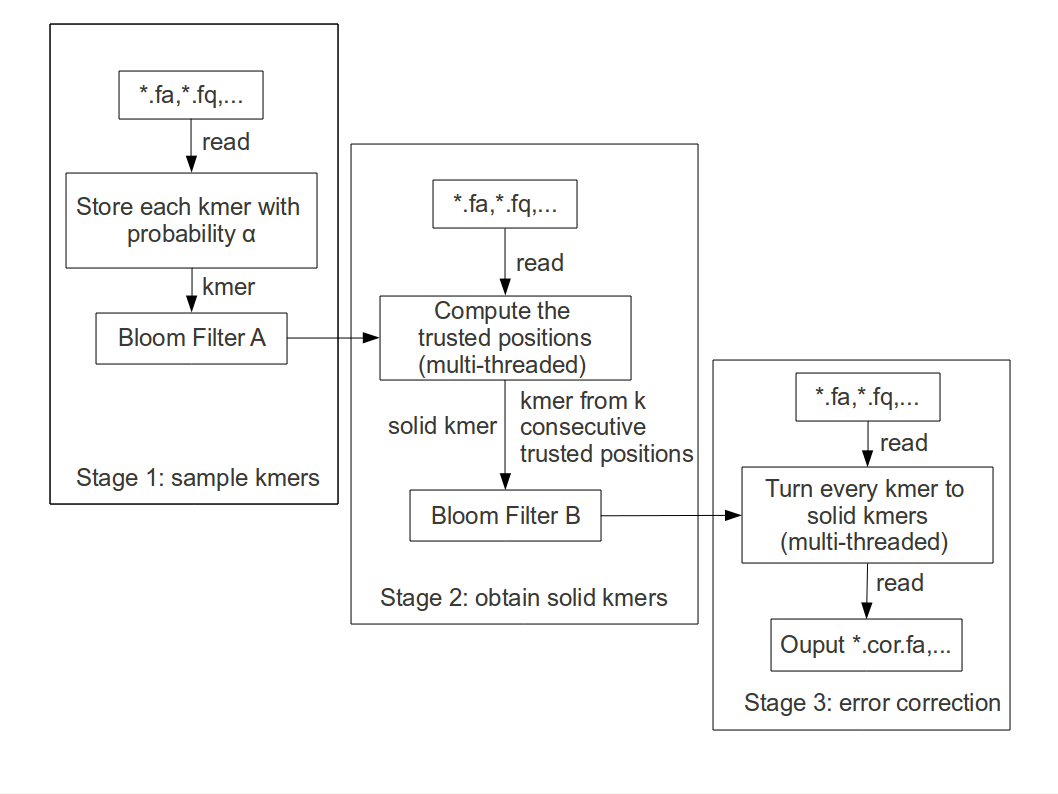
\includegraphics[width=0.75\textwidth]{lighter_framework.png}
\caption{The framework of Lighter\label{fig:lighter_framework}}
\end{center}
\end{figure}

\subsection*{Bloom filter}
A Bloom filter \cite{bloom1970space} is a compact probabilistic data structure representing a set.  It consists of an array of $m$ bits, initialized to 0.  To add an object $o$, $h$ independent hash functions $H_0(o), H_1(o),...,H_{h-1}(o)$ are applied.  Each maps $o$ to an integer in $[0, m)$ and the corresponding $h$ array bits are set to 1. To test if object $q$ is a member, the same hash functions are applied to $q$.  $q$ is a member if all corresponding bits are set to 1.  A false positive occurs when the corresponding bits are set to 1 ``by coincidence,'' that is, because of objects besides $q$ that were added previously.  Assuming the hash functions map objects to bit array elements with equal probability, the Bloom filter's false positive rate is approximately $(1-e^{-h\frac{n}{m}})^h$, where $n$ is the number of distinct objects added, also called the \emph{occupancy}.  Given $n$, which is usually determined by the dataset, $m$ and $h$ can be adjusted to achieve a desired false positive rate.  Lower false positive rates can come at a cost, since greater values of $m$ incur more memory usage and greater values of $k$ require more hash function calculations.  Many variations on Bloom filters have been proposed that additionally permit, for example, compression of the filter, storage of count data, representation of maps in addition to sets, etc \cite{tarkoma2012theory}.  Bloom filters and variants thereon have been applied in various bioinformatics settings, including assembly \cite{pell2012scaling}, compression \cite{jones2012compression}, k-mer counting \cite{melsted2011efficient}, and error correction \cite{shi2010parallel}.

By way of contrast, another way to represent a set is with a hash table.  These have the advantage of never yielding false positives.  But Bloom filters are far smaller.  Whereas a Bloom filter is an array of bits, a hash table is an array of buckets, each large enough to store a pointer, key, or both.  If chaining is used, lists associated with buckets incur additional overhead.  While the Bloom filter's small size comes at the expense of false positives, these can be tolerated in many settings including in error correction.

In our method, the objects to be stored in the Bloom filters are k-mers.  Because we would like to treat genome strands equivalently for counting purposes, we will always \emph{canonicalize} a k-mer before adding it to, or using it to query a Bloom filter.  A canonicalized k-mer is either the k-mer itself or its reverse complement, whichever is less than or equal to the other.

\subsection*{First pass: downsampling}

Consider a k-mer drawn from a read.  The k-mer is \emph{incorrect} if its sequence has been altered by one or more sequencing errors.  Otherwise it is \emph{correct}.  Others have noted that, given a dataset with deep and uniform coverage, incorrect k-mers occur rarely (usually just once) while correct k-mers occur many times, proportionally to coverage \cite{pevzner2001eulerian, chaisson2004fragment}.

In the first pass over the input reads, Lighter examines each k-mer of each read, canonicalizing and storing it in Bloom filter $A$ with probability $\alpha$, where $\alpha$ is an adjustable parameter.  Say a particular k-mer sequence occurs a total of $N_k$ times in the dataset.  If the $\alpha$ filter discards all $N_k$ occurrences, the k-mer is never added to $A$ and $A$'s occupancy is reduced by one.  Thus, reducing $\alpha$ in turn reduces $A$'s occupancy.  Because correct k-mers are more numerous, incorrect k-mers tend to be discarded from $A$ before correct k-mers as $\alpha$ decreases.  In the rest of the method, it is beneficial for $A$ to include as many correct and as few incorrect k-mers as possible, though the method is still robust when $A$ contains some incorrect and lacks some correct k-mers.

Assume that, regardless of average coverage, there is always a value of $\alpha$ for which $n \approx G$, where $G$ is the length of the sequenced genome, and the k-mers stored in $A$ are almost all correct.  If this is the case, we can fix $m$ and $h$ and adjust $\alpha$ to achieve a desired false positive rate.  This is in contrast to fixing $n$ and adjusting $m$ and $h$.  We do not argue here that the assumption is true, but we do show later that in practice $\alpha$ can be set to achieve desirable $m$, $k$ and false positive rate for a range of coverage levels.

%In other words, the size of $A$ depends almost only on the genome size. For $75\times$ coverage sequence data, we can let $\alpha$ be $0.05$.

\subsection*{Second pass: obtaining solid k-mers}

Let $m(r)$ denote the number of times $k$-mer $r$ occurs in the input reads.  We define a threshold $f$ such that a $k$-mer $r$ is considered \emph{weak} when $m(r) \leq f$.  Ignoring false positives, the following inequality bounds the probability $P(\alpha)$ that a particular weak $k$-mer appears in Bloom filter $A$ when the downsampling rate is $\alpha$:

\begin{equation}P(\alpha) \leq 1-(1-\alpha)^f\end{equation}

For each position in a read, it can affect up to $x$ kmers where $1\le x\le k$. If that position is wrong, these $x$ kmers will not show up many times and they are mostly likely not in $A$. Suppose, a kmer with frequency less than $f$ is very weak, then the probability of such kmer be in $A$ is less than $P=1-(1-\alpha)^f$. For the $x$ kmers containing the specific position, we can assume that the number of those stored in $A$ follows a binomial distribution with parameter $(x,P)$. We can decide whether the nucleotide of a position is trusted by one-tail hypothesis testing. The null hypothesis is that this position is wrong and the p-value can be get from test again $(x,P)$ using the actual number of kmers in $A$ containing that position. We use $y$ to denote this actual number of kmers. In our method, suppose $y'$ is the first number whose p-value is smaller than 0.005, if $y>y'$, we reject the null hypothes and the position is trusted. The benefit of using hypothesis testing instead of using a fixed threshold is that we can handle the case where $x<k$ in a uniform way and it can tolerate the ill-chosen $\alpha$. Notice that, the position near the left and right boundary or near the error may never be trusted.

To show that we can keep the size of $A$ nearly constant regardless of the coverage. Considering in one case 1, we have the coverage $C$. And in the next case 2, we double the coverage. Theoretically, the occurence time of error-free kmers should be doubled and so is the counting of the kmers showing up only one or two times. In case 1, we sample the kmers with probability $\alpha_1$, and $\alpha_2$ in case 2. In case 1, A kmer is solid if it showed up $t$ times; a kmer is weak if it showed up less than $f$ times. We can set $f$ is proportional to $t$ and is much smaller than $t$, like $t=0.05f$. So in case 2, a solid kmer showed up at least about $2t$ times while a weak kmer showed up at most about $2f$ times. If we want the same null hypothesis binomial distribution for the same position in these two cases, we need $P_1=P_2$ as the base, where $P_1=1-(1-\alpha_1)^f$, $P_2=1-(1-\alpha_2)^{2f}$.
$$P_2=1-(1-\alpha_2)^{2f}=1-(1-2\alpha_2+\alpha_2^2)^f=P_1=1-(1-\alpha_1)^f$$
$$\Leftrightarrow 1-2\alpha_2+\alpha_2^2=1-\alpha \Leftrightarrow \alpha_2=1 \pm \sqrt{1-\alpha_1}$$
Since $\alpha_2$ is no more than 1, $\alpha_2=1-\sqrt{1-\alpha_1}$

Similarly, we can show the same relationship for the hypothesis distribution, $P'_1$ and $P'_2$, where $P_1=1-(1-1-\alpha_1)^t$, $P_2=1-(1-1-\alpha_2)^{2t}$. So we can change the $\alpha$ to make the hypothesis testing from different coverage data set equivalent.

In practice, $\alpha_1$ is very small, so $\alpha_2$ is also very small. If we ignore this quadratic term $\alpha_2^2$, we have $\alpha_2=\alpha_1 / 2$. Considering the kmers showing up only once, they takes most of the space and the number of them sampled into table $A$ is the same in case 1 and 2 with parameter $\alpha_1$ and $\alpha_2/2$ respectively. This shows that our method has the property of keeping the space complexity near constant. 

After marking each positions, if there are consecutive k trusted positions, we store the corresponding kmer, which is called solid kmer, in another bloom filter $B$. Because these kmers are likely from the real genome, the size of $B$ also only depends on the genome size. 

In both table $A$ and $B$, we only store the cannonical form of a kmer, that is the kmer itself or its rever complement depending on who has smaller lexicographical order. We know that there is nearly linear relationship between $1/\alpha$ and $f$ the frequency for the weak kmers, in Lighter, we set $f=max\{2,0.1/\alpha\}$ and the user will choose $\alpha$. A rule of thumb for choosing $\alpha$ is by applying the nearly linear relationship between $1/\alpha$ and the coverage, and in this paper we choose $\alpha=0.05$ when the coverage is $70\times$. So given the coverage $C$, we can set $\alpha$ to $0.05\frac{70}{C}$. 

\subsection*{Third pass: error correction}
To show that our method of getting and storing solid kmers is reliable, we designed an error correction method just using the kmers stored in bloom filter $B$.

The correction is done read by read. For a read of length $|r|$, we have $|r|-k+1$ kmers and $k_i$ denote the kmer starts at position $i$ where $1\le i\le|r|-k+1$. We start the correction by finding a longest consecutive kmers that are stored in $B$, and then do the correction by scanning towards left and right. Since the correction towards left and right are symmetric, we only demonstrate the correction for the right-hand scanning. Ideally, when we move from the solid kmers towards right, the first time we see an weak kmer, say $k_i$, there must be an error at position $i+k-1$. There are three candidates or four(if the position is N) to replace this position. For each candidate, we see how many consecutive kmers is solid starting from $k_i$ with this new character. We choose the candidate creating most solid kmers. Then we resume scanning towards right starting from the next unstored kmer. If none of the candidate makes $k_i$ solid or more than one candidate create most solid kmers, we say position $i+k-1$ is ambiguous and stop there. If $i+k-1$ is far from the end of the read, we do the error correction on the substring from $i+k-1$ to the end of a read.

The scheme of this greedy error correction method is shown in Figure \ref{fig:error_correction}, where we choose found the error because there is no kmer CCGATTC. We choose A to replace C since it gives us most consecutive solid kmers up to the end of the read.

\begin{figure}[h!]
\begin{center}
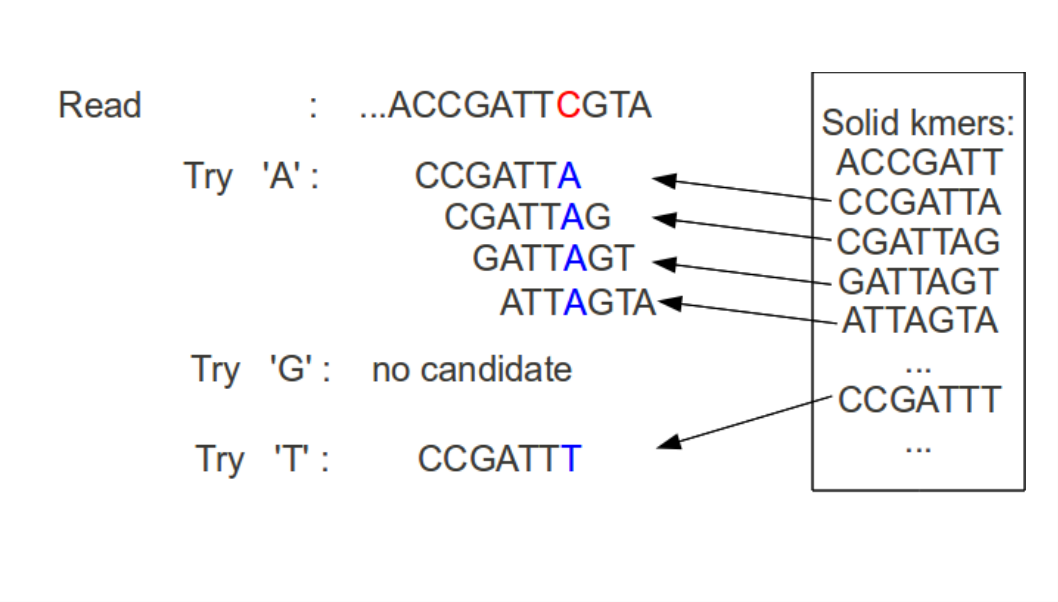
\includegraphics[width=0.75\textwidth]{ErrorCorrection.png}
\caption{The framework of Lighter\label{fig:error_correction}}
\end{center}
\end{figure}

\subsection*{Parallization}
As shown in Figure \ref{fig:lighter_framework}, Lighter works in three stages: sampling kmers, obtaining solid kmers and error correction. For the sampling kmers stage, because $\alpha$ is very small, most of the time is spent on scanning the reads namely reading the files. As a result, the overhead of parallilize this part will dominate the benefits, so we decide to remain this stage serial. In the second stage, each thread will handle different reads independently. Reading bloom filter in parallel is very efficient since there is no data race. When a thread find a solid kmer, it firstly tests whether this kmer is stored in table B or not. If this kmer is not in table B, then we write this kmer into the table. In this way, we can avoid many writing locks for table B because a solid kmer shows up many times. The thrid stage can parallized embarrsingly.

\section*{Evaluation}
\subsection*{Simulated data set}
We compared the our result with other released programs, Quake[cite], Musket[cite] and Bless[cite]. We use Mason[cite] to generate a set of data sets with ecoli as the reference genome. The K12 strain of ecoli is fully sequenced and has the decent length for us to generated different scenarios easily. 

In the simulated data set, we considered the coverage of $35$x, $75$x, $140$x, and the average error rate of $1\%$ and $3\%$. So there are totally 6 data sets. Because Mason can also specifiy the error rate of the first and the last base repsectively, suppose the average error rate is $e$, we set the error rate of the first base to $e/2$ and the error rate of the last base is $3e$. This setting is more realistic than a uniform error rate model. 
%TODO: define recall,...

We say a base is true positive(TP) if we identify the error and correct it into the right one; a base is false positive(FP) if we correct an original error-free base; a base is false negative(FN) if it is wrong and we either fail to detect its error or we make a wrong correction. As tradition[cite], we use four measurement to evaluate the error correction methods: recall=TP/(TP$+$NP), precision=TP/(TP$+$FP), F-score=2$\times$recall$\times$precision/(recall$+$precision) which is a kind of average of recall and precision and Gain=(TP-FP)/(TP+FN) which measure the benefit of using error correction.

% Insert the table here.
\mbox{
\begin{tabular}{|c|c|c|c|c|c|c|c|}\hline
Coverage &	& \multicolumn{2}{|c|}{$35\times$}  & \multicolumn{2}{|c|}{$70\times$} & \multicolumn{2}{|c|}{$140\times$} \\ \hline
Error rate & & $1\%$ & $3\%$ & $1\%$ & $3\%$ & $1\%$ & $3\%$ \\ \hhline{|=|=|=|=|=|=|=|=|}
	& quake	& 89.59	& 48.77	& 89.64	& 48.82	& 89.59	& 48.78 \\ \cline{2-8}
Recall	& musket	& 92.61	& 92.04	& 92.60	& 92.05	& 92.60	& 92.03 \\ \cline{2-8}
	& bless	& 98.68	& 97.29	& 98.69	& 97.48	& 98.65	& 97.47 \\ \cline{2-8}
	& lighter	& 99.40	& 97.99	& 99.33	& 98.71	& 99.37	& 98.87 \\ \hhline{|=|=|=|=|=|=|=|=|}
	& quake	& 99.99	& 99.99	& 99.99	& 99.99	& 99.99	& 99.99 \\ \cline{2-8}
Precision	& musket	& 99.78	& 99.63	& 99.78	& 99.63	& 99.78	& 99.63 \\ \cline{2-8}
	& bless	& 98.90	& 98.59	& 98.88	& 98.62	& 98.88	& 98.61 \\ \cline{2-8}
	& lighter	& 99.11	& 99.13	& 99.08	& 99.16	& 99.07	& 99.17 \\ \hhline{|=|=|=|=|=|=|=|=|}
	& quake	& 94.51	& 65.56	& 94.54	& 65.61	& 94.51	& 65.57 \\ \cline{2-8}
F-score	& musket	& 96.06	& 95.68	& 96.05	& 95.69	& 96.05	& 95.68 \\ \cline{2-8}
	& bless	& 98.79	& 97.94	& 98.78	& 98.04	& 98.77	& 98.04 \\ \cline{2-8}
	& lighter	& 99.25	& 98.56	& 99.20	& 98.94	& 99.22	& 99.02 \\ \hhline{|=|=|=|=|=|=|=|=|}
	& quake	& 89.58	& 48.76	& 89.64	& 48.82	& 89.59	& 48.78 \\ \cline{2-8}
Gain	& musket	& 92.40	& 91.70	& 92.39	& 91.71	& 92.39	& 91.69 \\ \cline{2-8}
	& bless	& 97.58	& 95.90	& 97.57	& 96.11	& 97.54	& 96.09 \\ \cline{2-8}
	& lighter	& 98.50	& 97.14	& 98.41	& 97.88	& 98.43	& 98.04 \\ \hhline{|=|=|=|=|=|=|=|=|}

\end{tabular}
}

The $\alpha$ value for the $35\times$, $70\times$, $140\times$ is $0.1$, $0.05$ and $0.025$ respectively. 

For Quake, we only measured the performance of the reported reads. Because Quake trimmed the untrusted tail of a read and throw away unfixable reads, it has a particularly high precision. But even if we only count the original errors in those reported reads, its sensitivity is very low. Lighter is among the best on different measurement and scenarios. This shows that our sampling method is able to distinguish most solid and weak kmer, and the error correction method is very effective.

We can show Lighter can achieve near constant space usage if the portion of set bits, namely occupancy rate, in the bloom filters stays almost the same. And this is true as shown in Table \ref{table:bloom_occupancy_coverage} given different coverages using simulated data set with 1\% error rate. When the coverage is very low, the occupancy rate in table $B$ is significant lower. This is because that when the coverage is very low, the count of the solid kmers is not very different from the weak kmers and the binomial test fails no matter how the $\alpha$ is set.

\begin{table}
\begin{tabular}{|c|c|c|}\hline
Coverage & Table A & Table B \\ \hline
$10\times$	& 42.21	& 23.21 \\ \hline
$20\times$	& 42.21	& 34.62  \\ \hline
$35\times$ & 41.35 & 35.33 \\ \hline
$70\times$ &41.37  &  35.44 \\ \hline
$140\times$ & 41.37	& 35.41 \\ \hline
$280\times$ & 41.37	& 35.44 \\ \hline
\end{tabular}
\caption{Occupancy rate(\%) for each table for different coverages\label{table:bloom_occupancy_coverage}}
\end{table}

To further test the performance of Lighter, we showed how many kmers from the reference genome is stored in table $B$. We used the simulated data with $70$x coverage and $1\%$ error rate. There are totally 4,553,699 distinct kmers from the genome on one strand, and 4,553,653 of them are in table $B$ which is almost all of them. We lose some kmers from the genome mostly due to the low coverage at the two ends of the chromosome.

The 6 simulated data sets are for haploid case, there are many species with a pair of chromosome in a cell, like human. Here we consider the case of diploid. We still use the e.coli genome as the reference genome and then introduce $0.1\%$ SNPs to generate the second reference genome. Mason then will sample the same amount of reads from the two genomes, totally form an $70$x coverage data set. There are 159,117 kmers containing the SNP position from one strand, and table $B$ holds 158,972 of them. Though the performance is not as good as haploid case, it still hold almost all of them. 

% test the performance of alpha
The sampling rate $\alpha$ is the key in Lighter which ensures the near constant space complexity. We did an evaluation on the simulated data set with $35\times$ coverage and $1\%$ error rate. And in this evaluation, we fix $f=2$ instead of $f=max\{2,0.1/\alpha\}$. The result is shown in Figure \ref{fig:alpha}.

\begin{figure}[h!]
\begin{center}
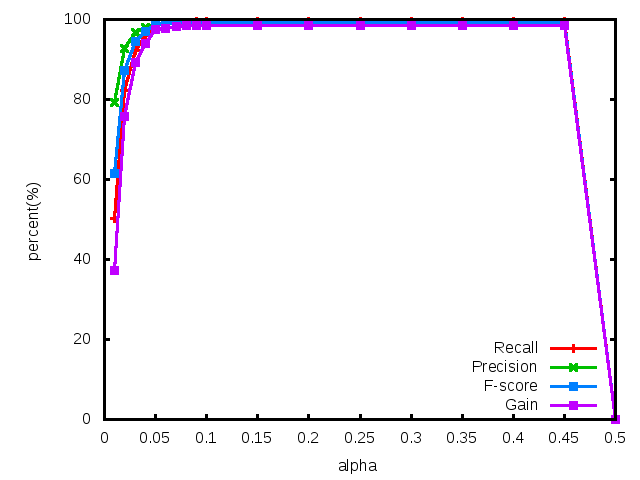
\includegraphics[width=0.5\textwidth]{alpha.png}
\caption{The effect of $\alpha$\label{fig:alpha}}
\end{center}
\end{figure}

If $\alpha$ is too small, too much solid kmers will be failed to get in table $A$ and too many positions will fail the hypothesis test. As a result, Lighter will try to correct those error-free region which also brings down the precision. And if $\alpha$ become even smaller, then there is no kmer in $B$, so Lighter will fail to correct all the reads because there is no candidate kmers. 

If $\alpha$ is larger, the hypothesis test is an adaptive threshold and handle this case nicely even if there are too many elements in $A$ and the false positive rate of $A$ is higher. However, when $\alpha$ is too large, number $k$ will have a p-value larger than 0.005, and all the positions will be regarded as untrusted. We can observe this from the dramatic drop in Figure \ref{fig:alpha}.

This explanation can also be verified by looking at the occupancy rate of table A and B from the simulated data sets with 3 different coverage and $1\%$ error rate when changing $\alpha$ shown in Figure \ref{fig:bloom_occupancy_alpha_all}. Also, we can see the occupancy rate of table A is almost the same given the same $\alpha\times\mbox{coverage}$ across the 3 data sets. And the occupancy rate of table B is very steady because the solid kmers from the genome are the same for the 3 data sets. When $\alpha$ is way too large than the optimal value, like in the $140\times$ data set, too much weak kmers get sampled and more likely to pass the binomial test which cause the failure of filtering non-solid kmers.

\begin{figure}[h!]
\begin{center}
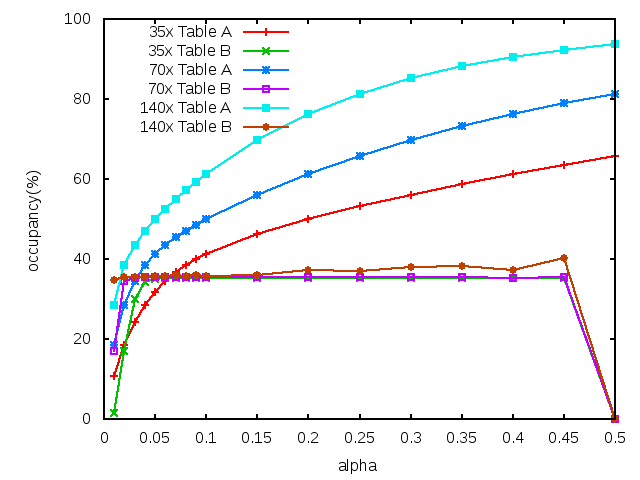
\includegraphics[width=0.5\textwidth]{bloom_occupancy_alpha_all.png}
\caption{The effect of $\alpha$ on occupancy rate\label{fig:bloom_occupancy_alpha_all}}
\end{center}
\end{figure}

\subsection*{Real data set}
\subsubsection*{E.Coli data set}
We use ERR022075 data set which is a very deep coverage sequencing data set of ecoli K-12 strain genome. We still used Quake, Musket, Bless and Lighter to run this data set. Since usually we do not need that much of coverage, we uniformly sampled some reads from this data set and got a data set with roughly 75x coverage. The reads in this data set is paired-end and the read length is 100 and 102. Because Bless can not handle paired-end reads with different length, we truncate the last 2 base to form a 100-length paired-end data set.

Since the genome of E.Coli K-12 strain is fully sequenced, we measured that 4,519,535 out of 4,553,699 kmers from the genome is stored in table $B$, which is more than $99\%$. This number can be slightly improved using larger $\alpha$. 
 
% Result of bowtie2
We can also measure the error corrections' affect on the alignment. We use Bowtie2[cite] to align the reads to the reference genome and count the total number of the matched position.

\begin{tabular}{|c|c|c|c|c|}\hline
  & Total Matched Pos & Improvement(\%) & Total pairs & Mapped \\ \hline
Original	& 343,081,567	& - & 1,748,808	& 99.04\% \\ \hline
Quake	& 327,813,255	& -4.45\%	& 1,684,792	& 99.98\% \\ \hline
Musket	& 345,403,149	& 0.68\%	& 1,748,808	& 99.15\% \\ \hline
Bless	& 345,947,230	& 0.84\%	& 1,748,808	& 99.30\% \\ \hline
Lighter	&  346,273,158 & 0.93\%	& 1,748,808	& 99.39\% \\ \hline
\end{tabular}

For Quake, the number is very low mainly due to unreported reads and trimmed 3' end. It turns out Lighter gives the most improvement. We use samtools to do the SNP calling. 

For those reads not got trimmed and alinged to the genome without indels (cigar field like 100M in the SAM file), we measure the matched ratio for each position shown in Figure \ref{fig:ecoli_perbase}. Since many of the reads in this data set start with N, the first base's matching ratio of the original data set is very low.

\begin{figure}[h!]
\begin{center}
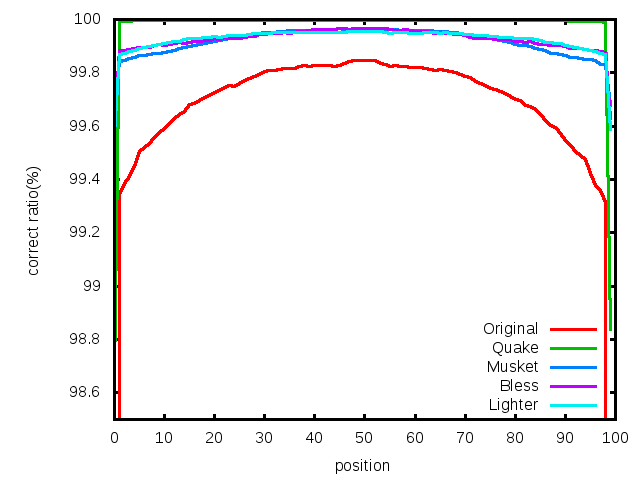
\includegraphics[width=0.5\textwidth]{per_base.png}
\caption{The matching ratio for each base in E.Coli data set\label{fig:ecoli_perbase}}
\end{center}
\end{figure}

% Result of SOAPDenovo2
Another common measurement for error correction is to run the de novo assembly and see the change of the N50 of the contigs and scaffolds. We use SOAPDenovo2[cite] to assemble the reads. SOAPDenovo2 is a de novo assembly software based on De Brujin graph. The parameter for SOAPDenovo2 especially the kmer size in the De Brujin graph is very important to the performance. We ran the SOAPdenovo2 on different parameters and choose the one with best N50 contig size. 

\begin{table}
\begin{tabular}{|c|c|c|} \hline
	  & contig N50 & scaffold N50 \\ \hline 
Original  &	53584	&	80924 \\ \hline 
Quake &	54854	&	89802 \\ \hline 
Musket&	47826	&	89873 \\ \hline 
Bless &	50573	&	84353 \\ \hline 
Lighter &	48777	&	86836 \\ \hline 
\end{tabular}
\caption{De novo assembly of E.Coli data set\label{table:ecoli_sd2}}
\end{table}

\subsubsection*{Human Chr14}
So far, we only tested the data on the genome of E.Coli, which is a pretty small. In this section, we use a data set from Gage[cite] on human chromosome 14. This data set is about 35x coverage and 101bp pair-end reads.

Like for the E.Coli data set, we evaluate the result using both Bowtie2 and SOAPdenovo2.

The result of Bowtie2 is shown in Table \ref{table:chr14_bowtie2}.

\begin{table}
\begin{tabular}{|c|c|c|c|c|}\hline
  & Total Matched Pos & Improvement(\%) & Total pairs & Mapped \\ \hline
Original &	3,581,034,345	&	& 18,252,400 & 98.60\% \\ \hline
Quake	& 3,040,192,216	& -15.10 &	16,280,259 &	99.96\% \\ \hline
Musket	& 3,631,477,901	& 1.41	& 18,252,400	& 99.38\% \\ \hline
Bless	& 3,636,682,539	& 1.55	& 18,252,400	& 99.43\% \\ \hline
Lighter	& 3,631,446,457	& 1.41	& 18,252,400	& 99.38\% \\ \hline
\end{tabular}
\caption{Alignment of chr14 data set\label{table:chr14_bowtie2}}
\end{table}

% Result of SOAPDenovo2
And the result 

\begin{table}
\begin{tabular}{|c|c|c|} \hline
		& contig N50	& scaffold N50 \\ \hline
Original	& 3372	& 9219 \\ \hline
Quake	& 3203	& 8727 \\ \hline
Musket	& 3760	& 6142 \\ \hline
Bless	& 3763	& 9254 \\ \hline
Lighter	&  3757	& 9012 \\ \hline
\end{tabular}
\caption{De novo assembly of chr14 data set\label{table:chr14}}
\end{table}

The results of the de novo assembly of the two real data set show that Lighter's result is comparable with other methods.

\subsection*{Running Time and Space Usage}
%describe the machine
The programs were run on a machine with 48 2.1GHz processors, 512G memory and 74T disk space. 

%The memory or disk usage from different programs 
Musket, Bless and Lighter are all aimming for low memory consumption. So we compared the peak memory usage as well as the peak disk consumption on the simulated data set with different coverage and with $1\%$ error rate and the chr14 real data from Gage.

\begin{tabular}{|c|c|c||c|c||c|c||c|c|} \hline
		& \multicolumn{2}{|c||}{$35\times$} & \multicolumn{2}{|c||}{$70\times$}  & \multicolumn{2}{|c||}{$140\times$} & \multicolumn{2}{|c|}{chr14}  \\ \hline
		& memory & disk & memory & disk & memory & disk & memory & disk \\ \hline
Quake   & 2.8G	& 3.3G & 7.1G & 6.0G & 14G & 12G & 48G & 57G \\ \hline		
Musket	& 139M	& 0 & 160M & 0 & 241M & 0 & 1.9G & 0 \\ \hline
Bless	& 10M	& 661M & 11M & 1.3G & 13M & 2.6G & 600M & 15G \\ \hline
Lighter	& 26M	& 0 & 26M & 0 & 26M & 0 & 354M & 0 \\ \hline
\end{tabular}

From the table, we can see that Bless and Lighter can achieve nearly constant memory consumption as claimed. Musket took much less memory comparing with Quake but is much worse than Bless and Lighter.

For Bless, we increase the number of temporary files along with the coverage of the data set to achieve the constant memory consumption. Bless uses secondary memory to save the memory consumption, and the overall space consumption is much larger than Musket and Lighter. 

For the chr14 data set, The memory consumption of Bless can be decreased if we create more temporary files. 

%runtime on simulated_70_1
We compared the running time between Quake, Musket and Lighter using different number of threads on the simulated data set with $70\times$ coverage and $1\%$ error in Figure \ref{fig:runtime}. Musket requires at least 2 threads due to its master-slave style parallelism, so its figure start at when number of threads is 2. 

\begin{figure}[h!]
\begin{center}
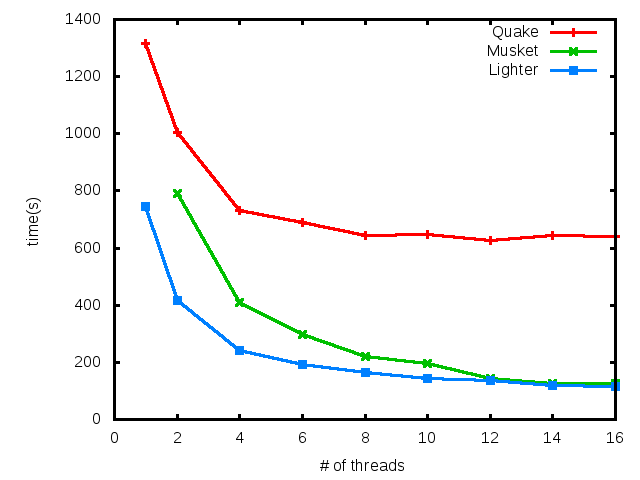
\includegraphics[width=0.5\textwidth]{runtime.png}
\end{center}
\caption{The running time on simulated data set with different number of threads\label{fig:runtime}}
\end{figure}

So far, Bless can only run in single-thread mode and it takes 1475s to finish which is much slower than Musket and Lighter.

The result shows that Lighter is very efficient and scalable. 

\section*{Discussion}
In this paper, we propose a probabilitic method of obtaining solid kmers without counting. It is the first method that is able to find solid kmer with near constant space complexity and it is very easy to implement.

We use this method to implement an error correction program Lighter for DNA-seq reads. As we expect, Light is space-efficient . Moreover, it is very fast and gives performance is comparable with other programs. This shows that our method of finding solid kmer is quite reliable. 

Another immediate application of our method is getting solid kmers' count, which can be done by scanning the reads again to get the real count for the solid kmers stored in table $B$. 

Since our method is probabilitic, we may miss few important information. Nevertheless, our method is extremely useful for programs like Quip[cite], where the accurate error correction is not critical. Even more, programs like Quip may directly use the solid kmers get by our method to do the assembly.

In this paper, we did not analyze the affect of $\alpha$ analytically and it is a difficult problem. So far, the size of table $A$ and $B$ are setting by considering unpractical pessimestic scenarios. If we know the effect in some compact form, we can optimize the performance of obtaining solid kmers by setting the best $\alpha$ and also use less space.

%%%%%%%%%%%%%%%%%%%%%%%%%%%
\section*{Acknowledgements}
  Text for this section \ldots

\bibliographystyle{abbrv}
\bibliography{lighter_paper}

\end{document}







